\section{Results}

\begin{figure}[t]
  \centering
  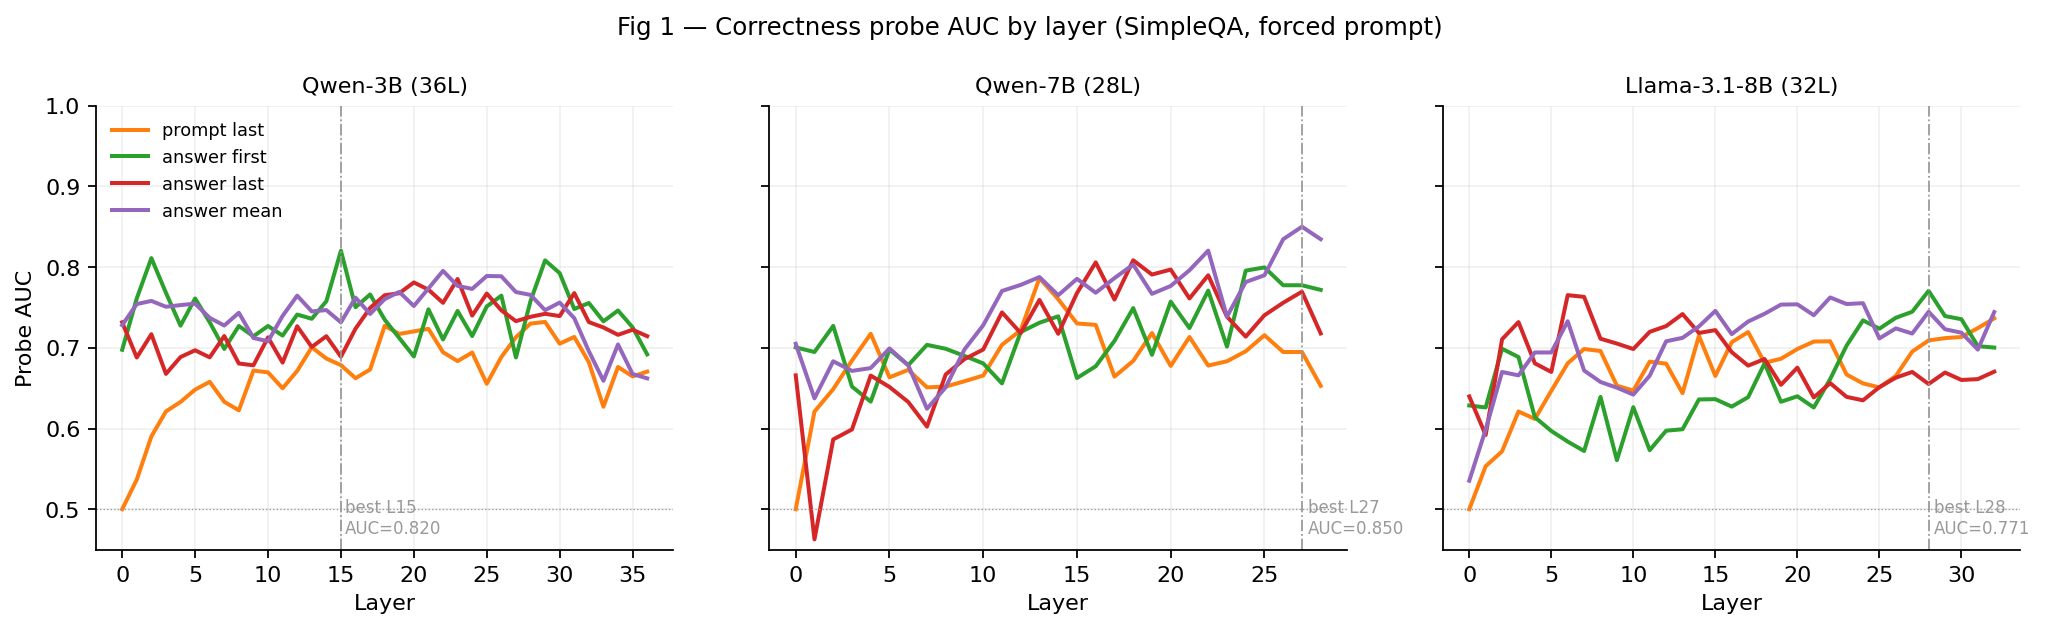
\includegraphics[width=0.9\linewidth]{fig1_probe_auc_by_layer.png}
  \caption{Probe AUC by layer and token position.}
  \label{fig:probe_auc}
\end{figure}

Internal correctness is readable from mid-to-late residual-stream states. Across
datasets, the best probe AUCs are strongest for PopQA, TriviaQA, SimpleQA,
TruthfulQA, and NQ-Open forced-answer settings.

\begin{figure}[t]
  \centering
  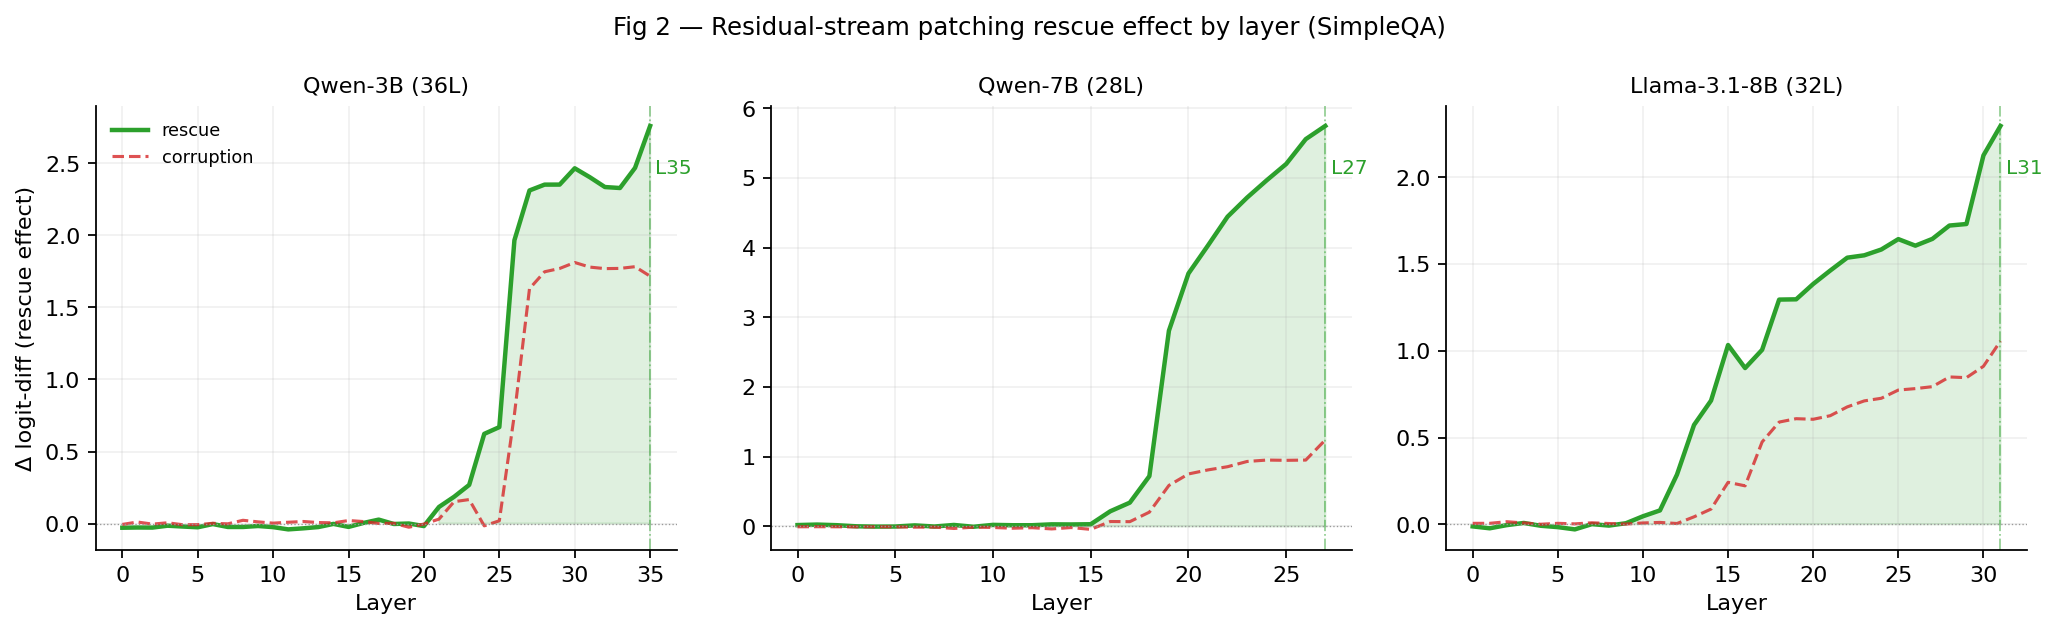
\includegraphics[width=0.9\linewidth]{fig2_rescue_by_layer.png}
  \caption{Activation patching rescue effect by layer.}
  \label{fig:rescue}
\end{figure}

Activation patching shows that late-layer states have causal influence on answer
selection. For Qwen2.5-3B-Instruct, rescue effects peak in the final layers,
while early layers have little effect.

\begin{figure}[t]
  \centering
  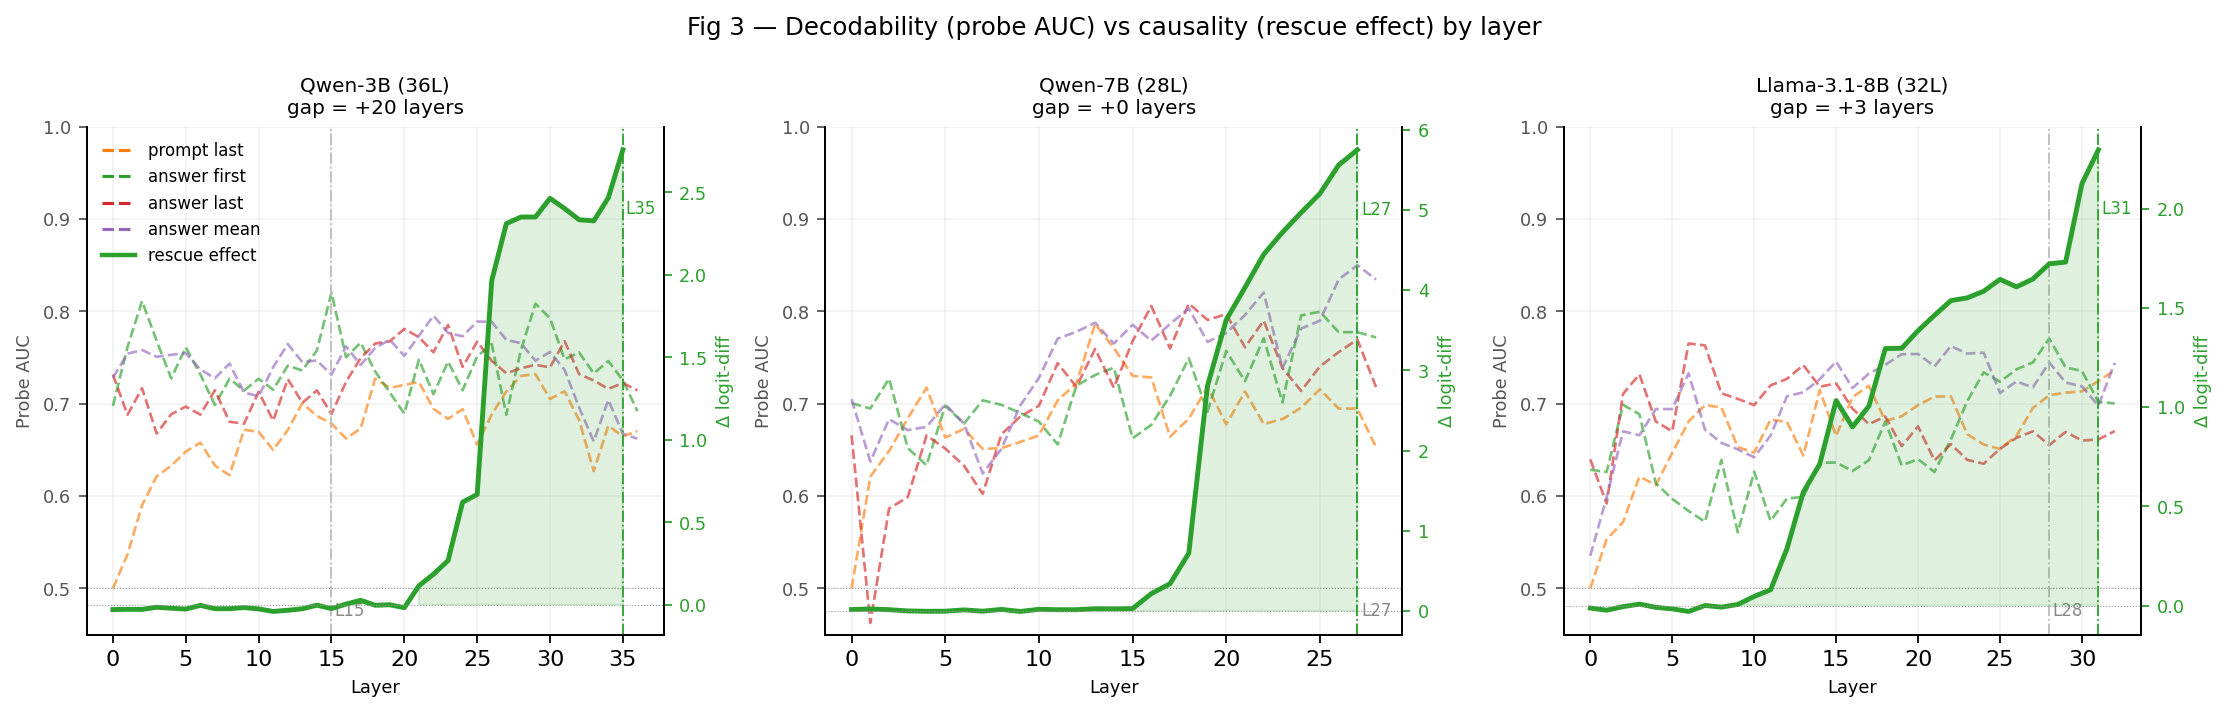
\includegraphics[width=0.9\linewidth]{fig3_decodability_vs_causality.png}
  \caption{Decodability and causal rescue peak at different layers.}
  \label{fig:decoda_causa}
\end{figure}

The most readable layer is not always the most causal layer. In Qwen2.5-3B,
correctness is most decodable around layer 15, but causal rescue peaks around
layer 35.

\begin{figure}[t]
  \centering
  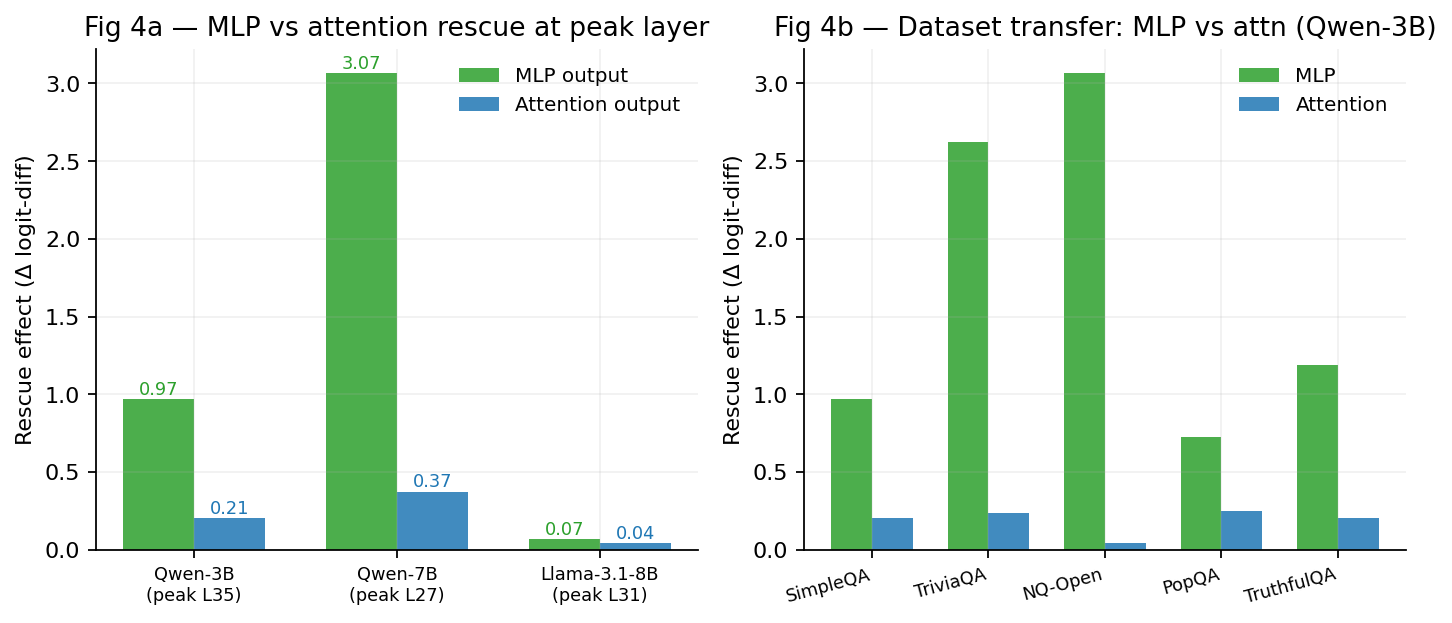
\includegraphics[width=0.9\linewidth]{fig4_component_localization.png}
  \caption{Late-layer MLP outputs dominate attention outputs in causal patching.}
  \label{fig:component}
\end{figure}

Component patching localizes most of the causal rescue effect to MLP outputs
rather than attention outputs. This pattern is observed across datasets and
replication models.

\begin{figure}[t]
  \centering
  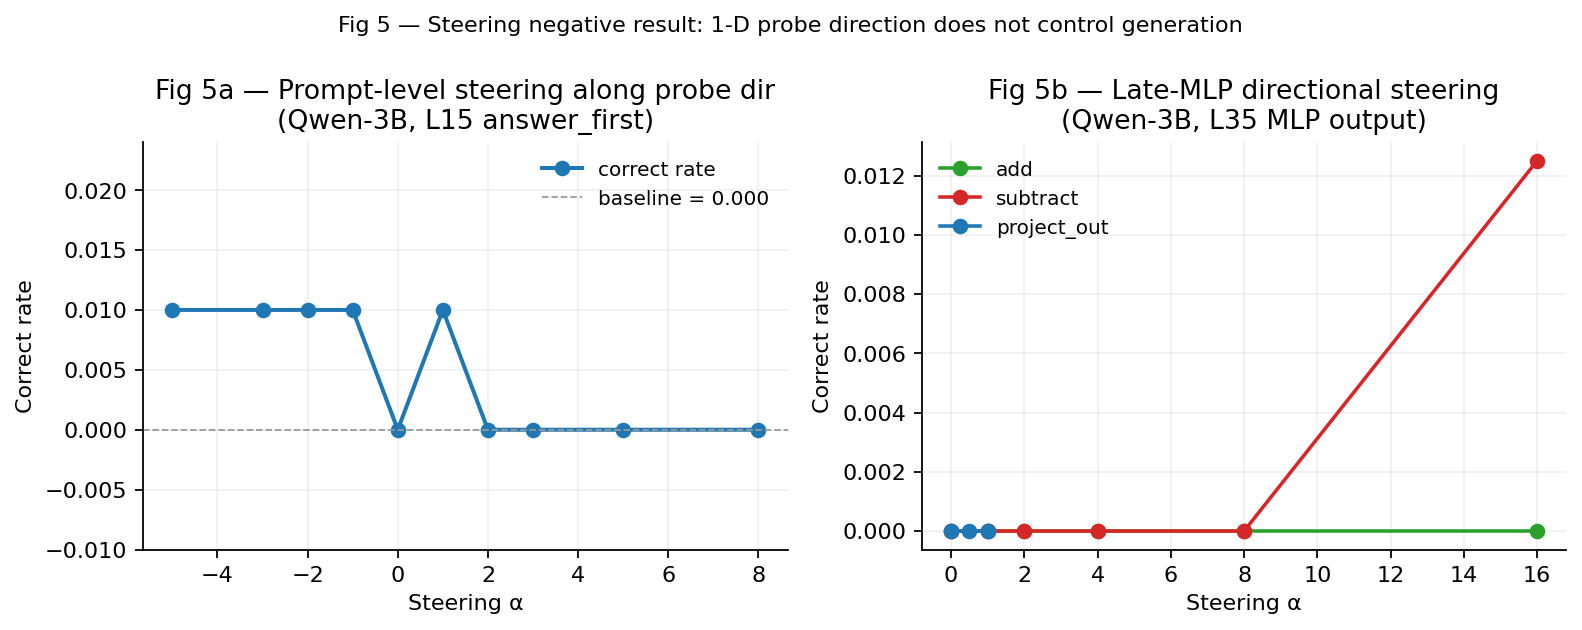
\includegraphics[width=0.9\linewidth]{fig5_steering_negative.png}
  \caption{Directional steering along a one-dimensional probe direction does not
  reliably improve correctness.}
  \label{fig:steering}
\end{figure}

Directional steering along the correctness probe direction has little effect on
answer correctness. The signal is readable, but a single linear direction is not
a sufficient control knob.

\begin{figure}[t]
  \centering
  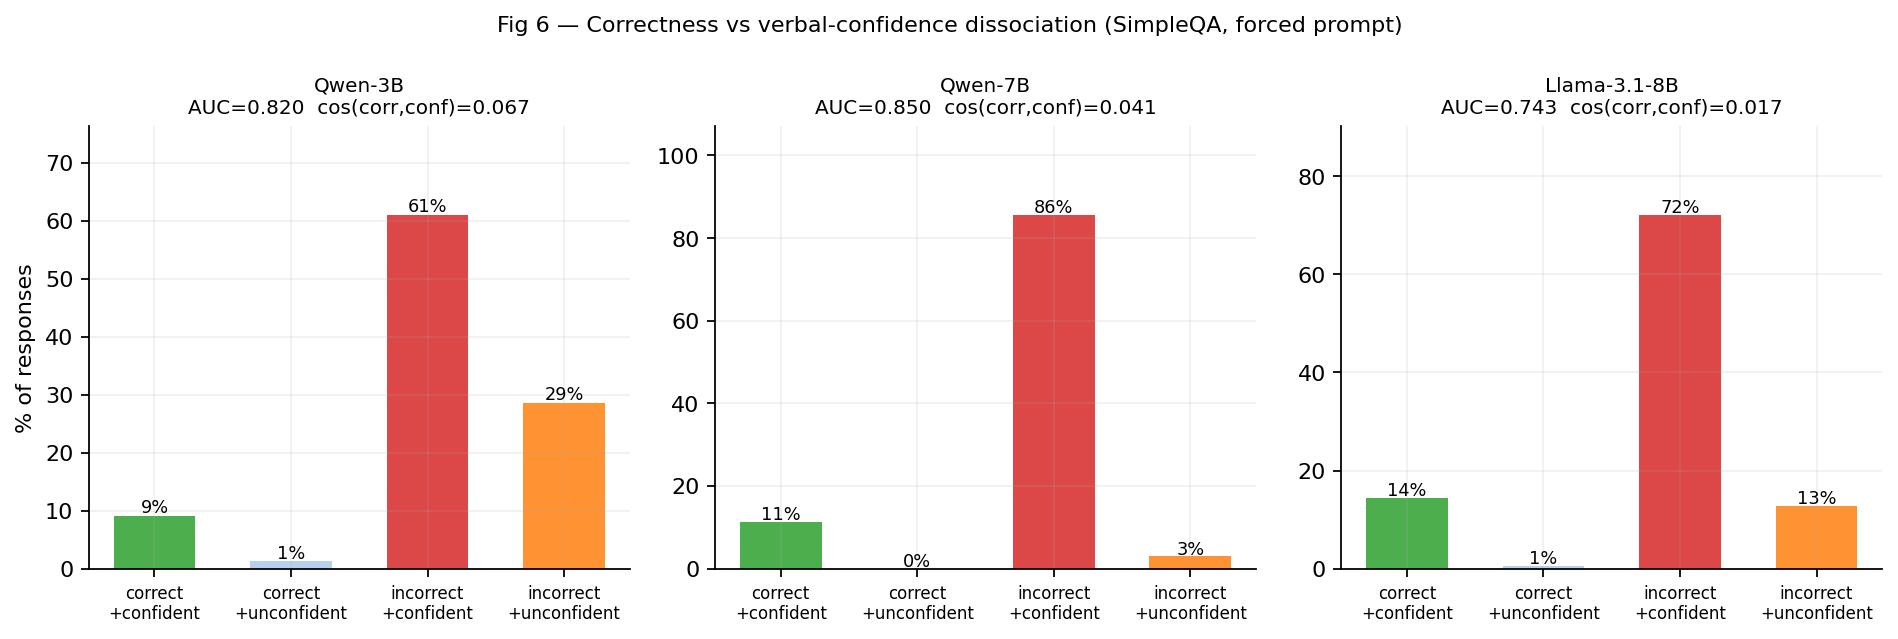
\includegraphics[width=0.9\linewidth]{fig6_confidence_dissociation.png}
  \caption{Correctness and verbal-confidence directions are nearly orthogonal.}
  \label{fig:confidence}
\end{figure}

Correctness and verbalized confidence are represented differently. Their probe
directions are nearly orthogonal, and many forced-answer generations are
incorrect while still receiving high verbal-confidence scores.

\begin{figure}[t]
  \centering
  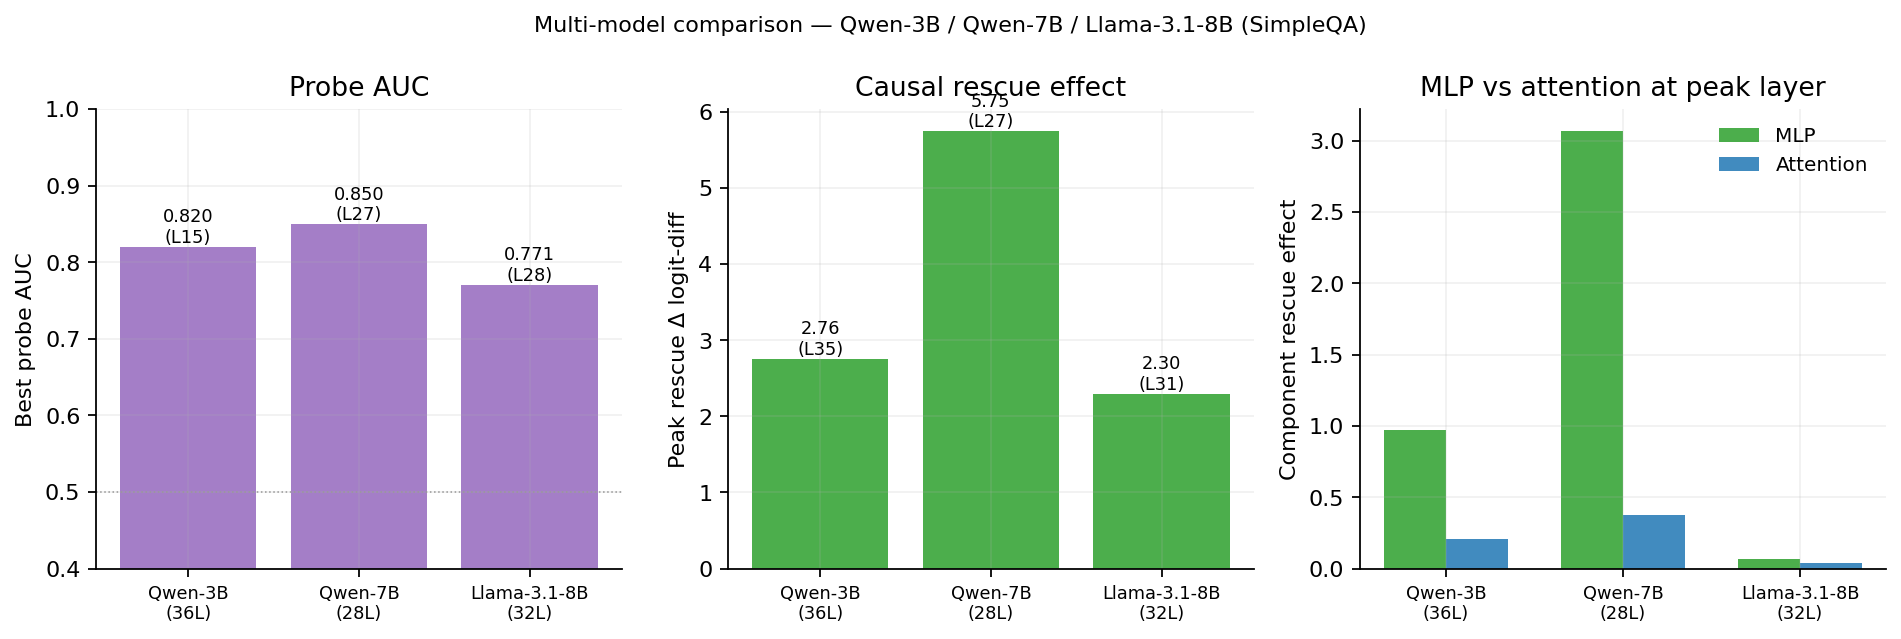
\includegraphics[width=0.9\linewidth]{fig_multimodel.png}
  \caption{Replication across Qwen2.5-3B, Qwen2.5-7B, and Llama-3.1-8B.}
  \label{fig:multimodel}
\end{figure}

The main pattern replicates across model families: correctness is decodable from
hidden states, late-layer patching has causal effects, and MLP outputs dominate
attention outputs at the causal bottleneck.
